\section{Virtual Analog Synthesis}

Virtual analog synthesis is the term used to describe the emulation of analog synthsizers of the 60s and 70s digitally in real time. The complexity and goals of an emulation can vary. Some emulations go so far as to simulate the actual electronic components of vintage synthesis circuits, others just model ths signal flow loosly.

Regardless of the type of emulation, and model of analog systhesis has two primary concerns. Latency and aliasing. The problem of latency has already been described above. Any processing will introduce a delay in the signal, the complexity of the processing can increase the delay, or use more CPU cycles. Aliasing is audible distortion introduced by signals that have a higher frequency content than the sampling rate of the system allows for\cite{virtual_analog_synthesis}.

Analog synthsizers usually employed what is refered to as subtractive synthsis. One or more sound generators or oscillators would create signals with particular harmonic qualities. These signals would then go through filters that would "subtract" frequencies from the signal. The oscillators and filters can be modulated as well as the amplitude of the filtered signal. Here is a simple block diagram of a typical subtractive synth voice.

\begin{figure}[p]
    \centering
    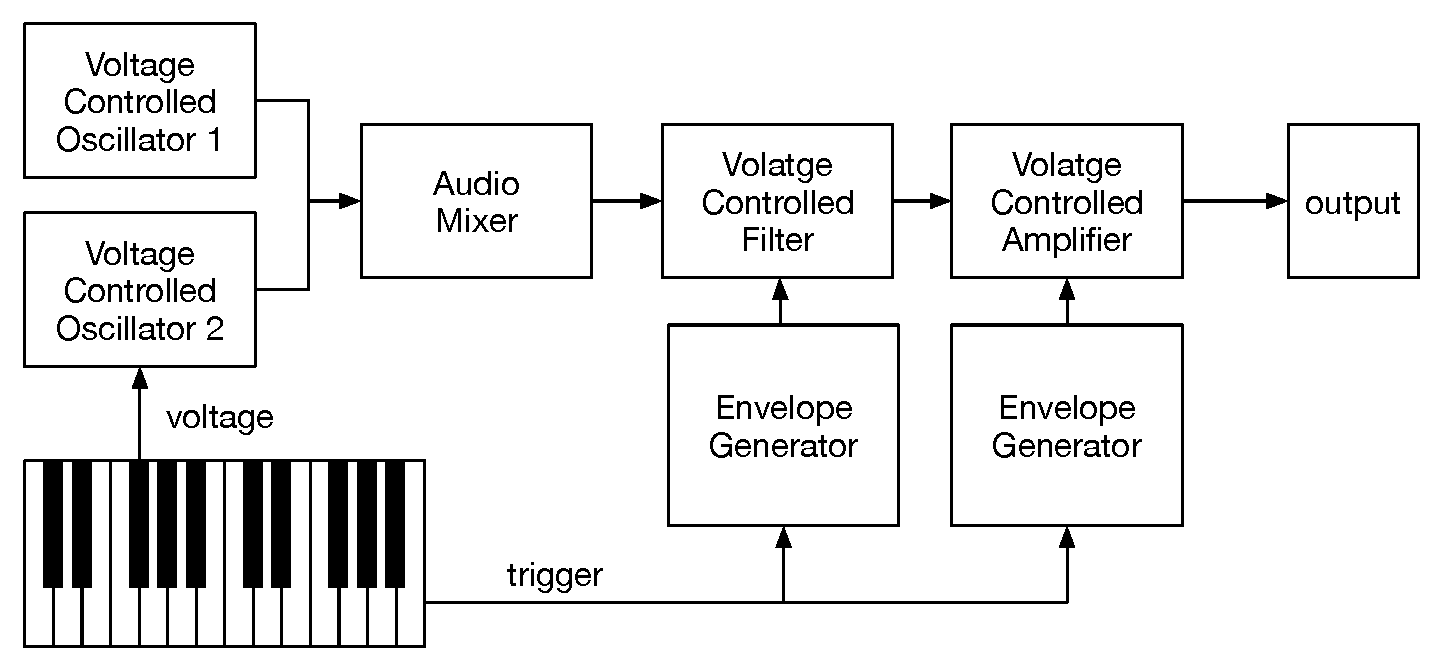
\includegraphics[width=\textwidth]{assets/synth_voice_block.pdf}
    \caption{Block Diagram of a Subtractive Synthesis Voice}
    \label{fig:synth_voice_block}
\end{figure}

The voltage controlled oscillators generate simple waveforms at the pitch coresponding to the note played on the keyboard.